\documentclass{beamer}


\usetheme{Warsaw}
\usecolortheme{crane}


\title{Power Series}
\subtitle{Mathematical Methods in the Physical Sciences}
\author{Steve Mazza}
\institute[Naval Postgraduate School]
{
  Naval Postgraduate School \\
  Monterey, CA \\
  
\includegraphics[height=3cm]{images/NPS_logo.jpg}
}
\date {SE3030, Winter/2014 \\ Quantitative Methods of Systems Engineering}
\subject{Quantitative Methods of Systems Engineering}


\begin{document}

\frame{\titlepage}

\begin{frame}{Introduction}
	Power series are series where the $n^{\mbox{th}}$ term is a constant times $x^n$ or a constant times $(x-a)^n$ where $a$ is also constant.
	\begin{block}{Definition}
		\begin{align*}
		\sum\limits_{n=0}^\infty a_nx^n&=a_0+a_1x+a_2x^2+a_3x^3+\cdots \\
		\sum\limits_{n=0}^\infty a_n(x-a)^n&=a_0+a_1(x-a)+a_2(x-a)^2+a_3(x-a)^3+\cdots
		\end{align*}
	\end{block}
\end{frame}

\frame{{Examples}
	The following are two of the examples that can also be found in Boas: \emph{Quantitative Methods of Systems Engineering} on page 20.
	\begin{exampleblock}{Example \#1}
		\[
		x-\dfrac{x^2}{2}+\dfrac{x^3}{3}-\dfrac{x^4}{4}+\cdots+\dfrac{(-1)^{x+1}x^n}{n}+\cdots 
		\]
	\end{exampleblock}
	\begin{exampleblock}{Example \#2}
		\[
		1+\dfrac{(x+2)}{\sqrt{2}}+\dfrac{(x+2)^2}{\sqrt{3}}+\cdots+\dfrac{(x+2)^n}{\sqrt{(n+1)}}+\cdots
		\]
	\end{exampleblock}
}

\begin{frame}{Interval of Convergence}
	Convergence of the power series depends on the value of $x$.  We can use the ratio test to find $x$ such that the series converges. 
\end{frame}
  
\begin{frame}{Theorems About Power Series}
\end{frame}
  
\begin{frame}{Expanding Functions in Power Series}
\end{frame}
  
\begin{frame}{Techniques for Obtaining Power Series Expansions}
    We outlay and demonstrate several methods of obtaining power series expansions.
    \begin{itemize}
    	\item Multiplying a series by polynomial or by another series
	\item Division of two series or of a series by a polynomial
	\item Binomial series
	\item Substitution of a polynomial or series or the variable in another series
	\item Combination of methods
	\item Taylor series using the basic Maclaurin series
	\item Using a computer
    \end{itemize}
\end{frame}
  
\begin{frame}{Techniques for Obtaining Power Series Expansions}
    \framesubtitle{Multiplying a Series by a Polynomial or by Another Series}
\end{frame}
  
\begin{frame}{Techniques for Obtaining Power Series Expansions}
    \framesubtitle{Division of Two Series or of a Series by a Polynomial}
\end{frame}
  
\begin{frame}{Techniques for Obtaining Power Series Expansions}
    \framesubtitle{Binomial Series}
\end{frame}
  
\begin{frame}{Techniques for Obtaining Power Series Expansions}
    \framesubtitle{Substitution of a Polynomial or a Series for the Variable in Another Series}
\end{frame}
  
\begin{frame}{Techniques for Obtaining Power Series Expansions}
    \framesubtitle{Combination of Methods}
\end{frame}
  
\begin{frame}{Techniques for Obtaining Power Series Expansions}
    \framesubtitle{Taylor Series Using the Basic Maclaurin Series}
    The Maclaurin series provides us with an alternative method to the formulas for obtaining a Taylor series.
   \begin{exampleblock}{Maclaurin Series}
       	\center{
       	    $\mbox{ln\ } x = \mbox{ln\ }[1+(x-1)]$
        }
   \end{exampleblock}
   Then we replace $x$ with $(x-1)$
   \begin{exampleblock}{Substitution}
   	\begin{align*}
   	    \mbox{ln\ } x&= \mbox{ln\ } [1+(x-1)] \\
	    &= (x-1)-\dfrac{1}{2}(x-1)^2+\dfrac{1}{3}(x-1)^3-\dfrac{1}{4}(x-1)^4\cdots
	\end{align*}
   \end{exampleblock}
\end{frame}
  
\begin{frame}{Techniques for Obtaining Power Series Expansions}
    \framesubtitle{Using a Computer}
\end{frame}
  
\begin{frame}{Accuracy of Series Approximations}
\end{frame}
  
\begin{frame}{Some Uses of Series}
\end{frame}

\begin{frame}{Example of columns 1}
    \begin{columns}[c] % the "c" option specifies center vertical alignment
    \column{.5\textwidth} % column designated by a command
     Contents of the first column
    \column{.5\textwidth}
     Contents split \\ into two lines
    \end{columns}
\end{frame}
 
\begin{frame}{Example of columns 2}
     \begin{columns}[t] % contents are top vertically aligned
     \begin{column}[T]{5cm} % each column can also be its own environment
     Contents of first column \\ split into two lines
     \end{column}
     \begin{column}[T]{5cm} % alternative top-align that's better for graphics
          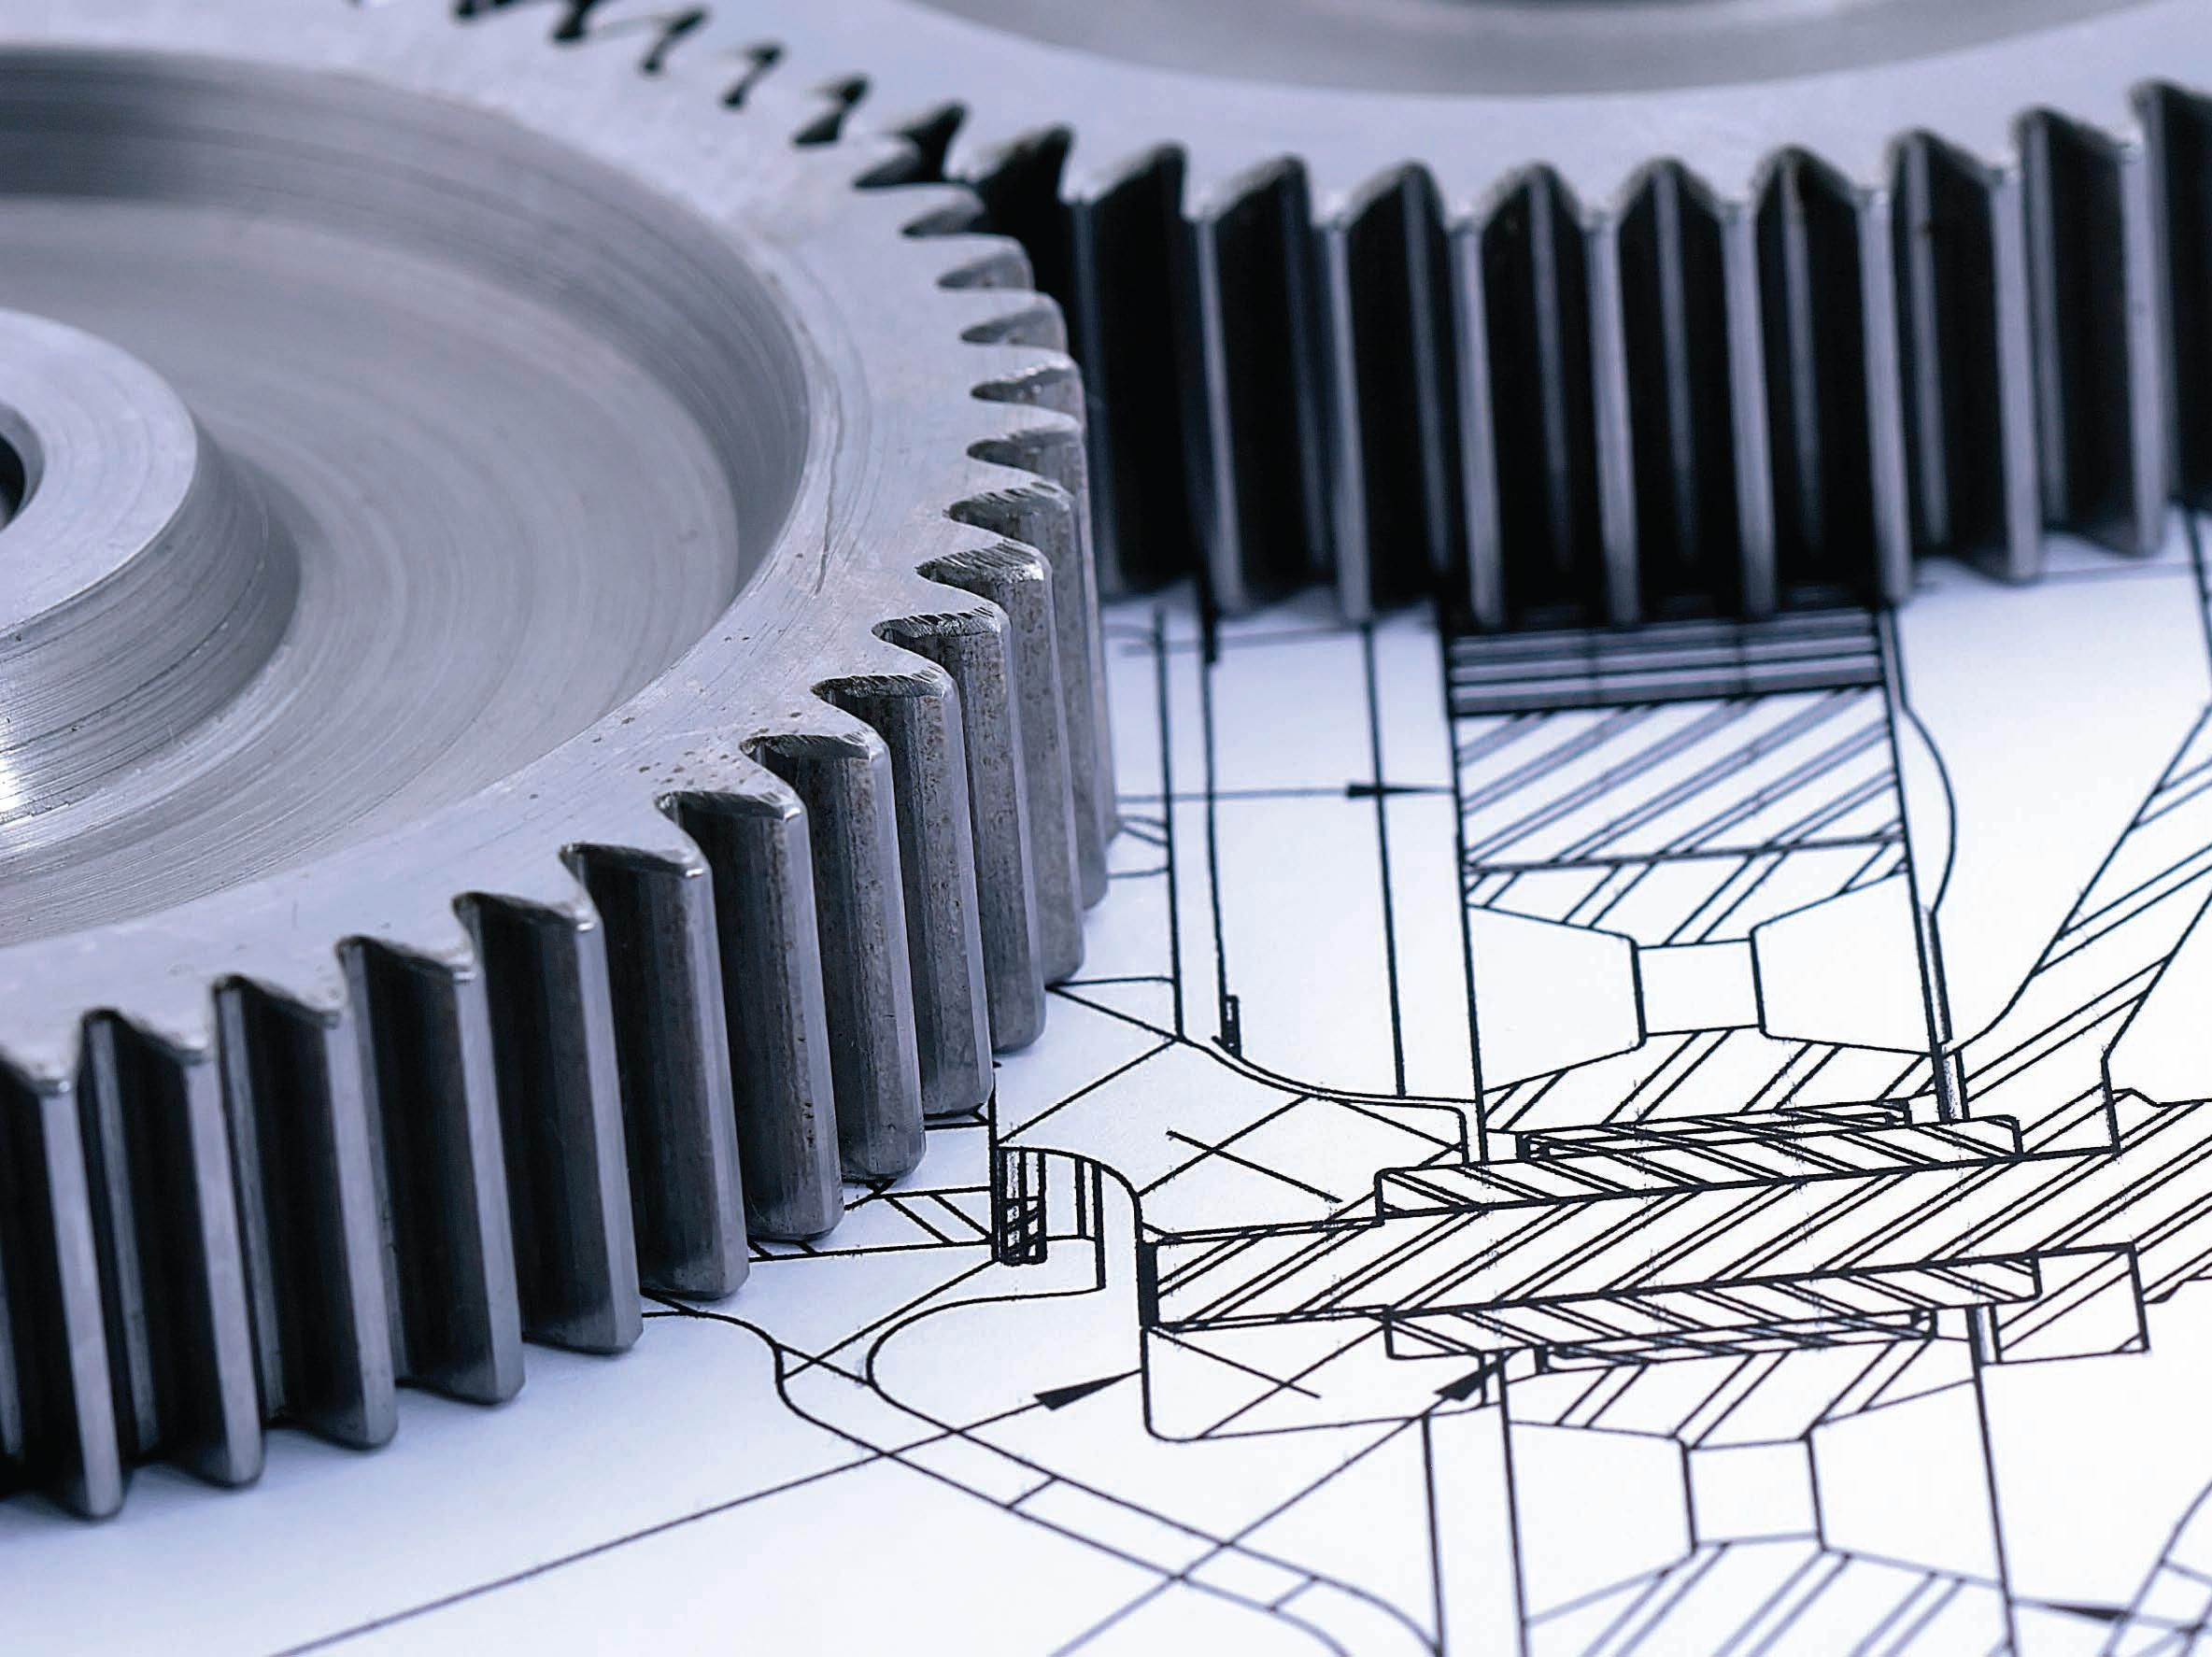
\includegraphics[height=3cm]{images/engineering.jpg}
     \end{column}
     \end{columns}
\end{frame}

\begin{frame}{Block Types}
   \begin{block}{This is a Block}
      This is important information
   \end{block}
 
   \begin{alertblock}{This is an Alert block}
   This is an important alert
   \end{alertblock}
 
   \begin{exampleblock}{This is an Example block}
   This is an example 
   \end{exampleblock}
\end{frame}

\end{document}
